\documentclass{article}%
\usepackage[T1]{fontenc}%
\usepackage[utf8]{inputenc}%
\usepackage{lmodern}%
\usepackage{textcomp}%
\usepackage{lastpage}%
\usepackage{graphicx}%
%
\usepackage[headheight=20pt, top=2cm]{geometry}%
\title{Analysis report for the "gag" gene in 9 supposedly alike sequences from a database}%
\author{Luis Jimenez}%
\date{\today}%
%
\begin{document}%
\normalsize%
\maketitle%
\section{Introduction}%
\label{sec:Introduction}%
The analyzed sequence extracted from GeneBank is OR876739.1, and the sequences used for the comparison by \%GC content were extracted from a database only with genomes that have the target gene, which are as follows: KP860667.1, KP860668.1, KP860669.1, KP860670.1, PP483791.1, PP483792.1, PP483793.1, PP483794.1, PP483795.1. Additionally, a comprehensive BLASTN analysis against the database was executed to calculate the percentage identity, suggesting potential validation of the target sequence's similarity to those from the database.

%
\section{Graphic comparison via GC content}%
\label{sec:GraphiccomparisonviaGCcontent}%
\subsection{Density of \% GC Content and \% GC Content for the randomized sequences}%
\label{subsec:DensityofGCContentandGCContentfortherandomizedsequences}%


\begin{figure}[!htbp]%
\centering%
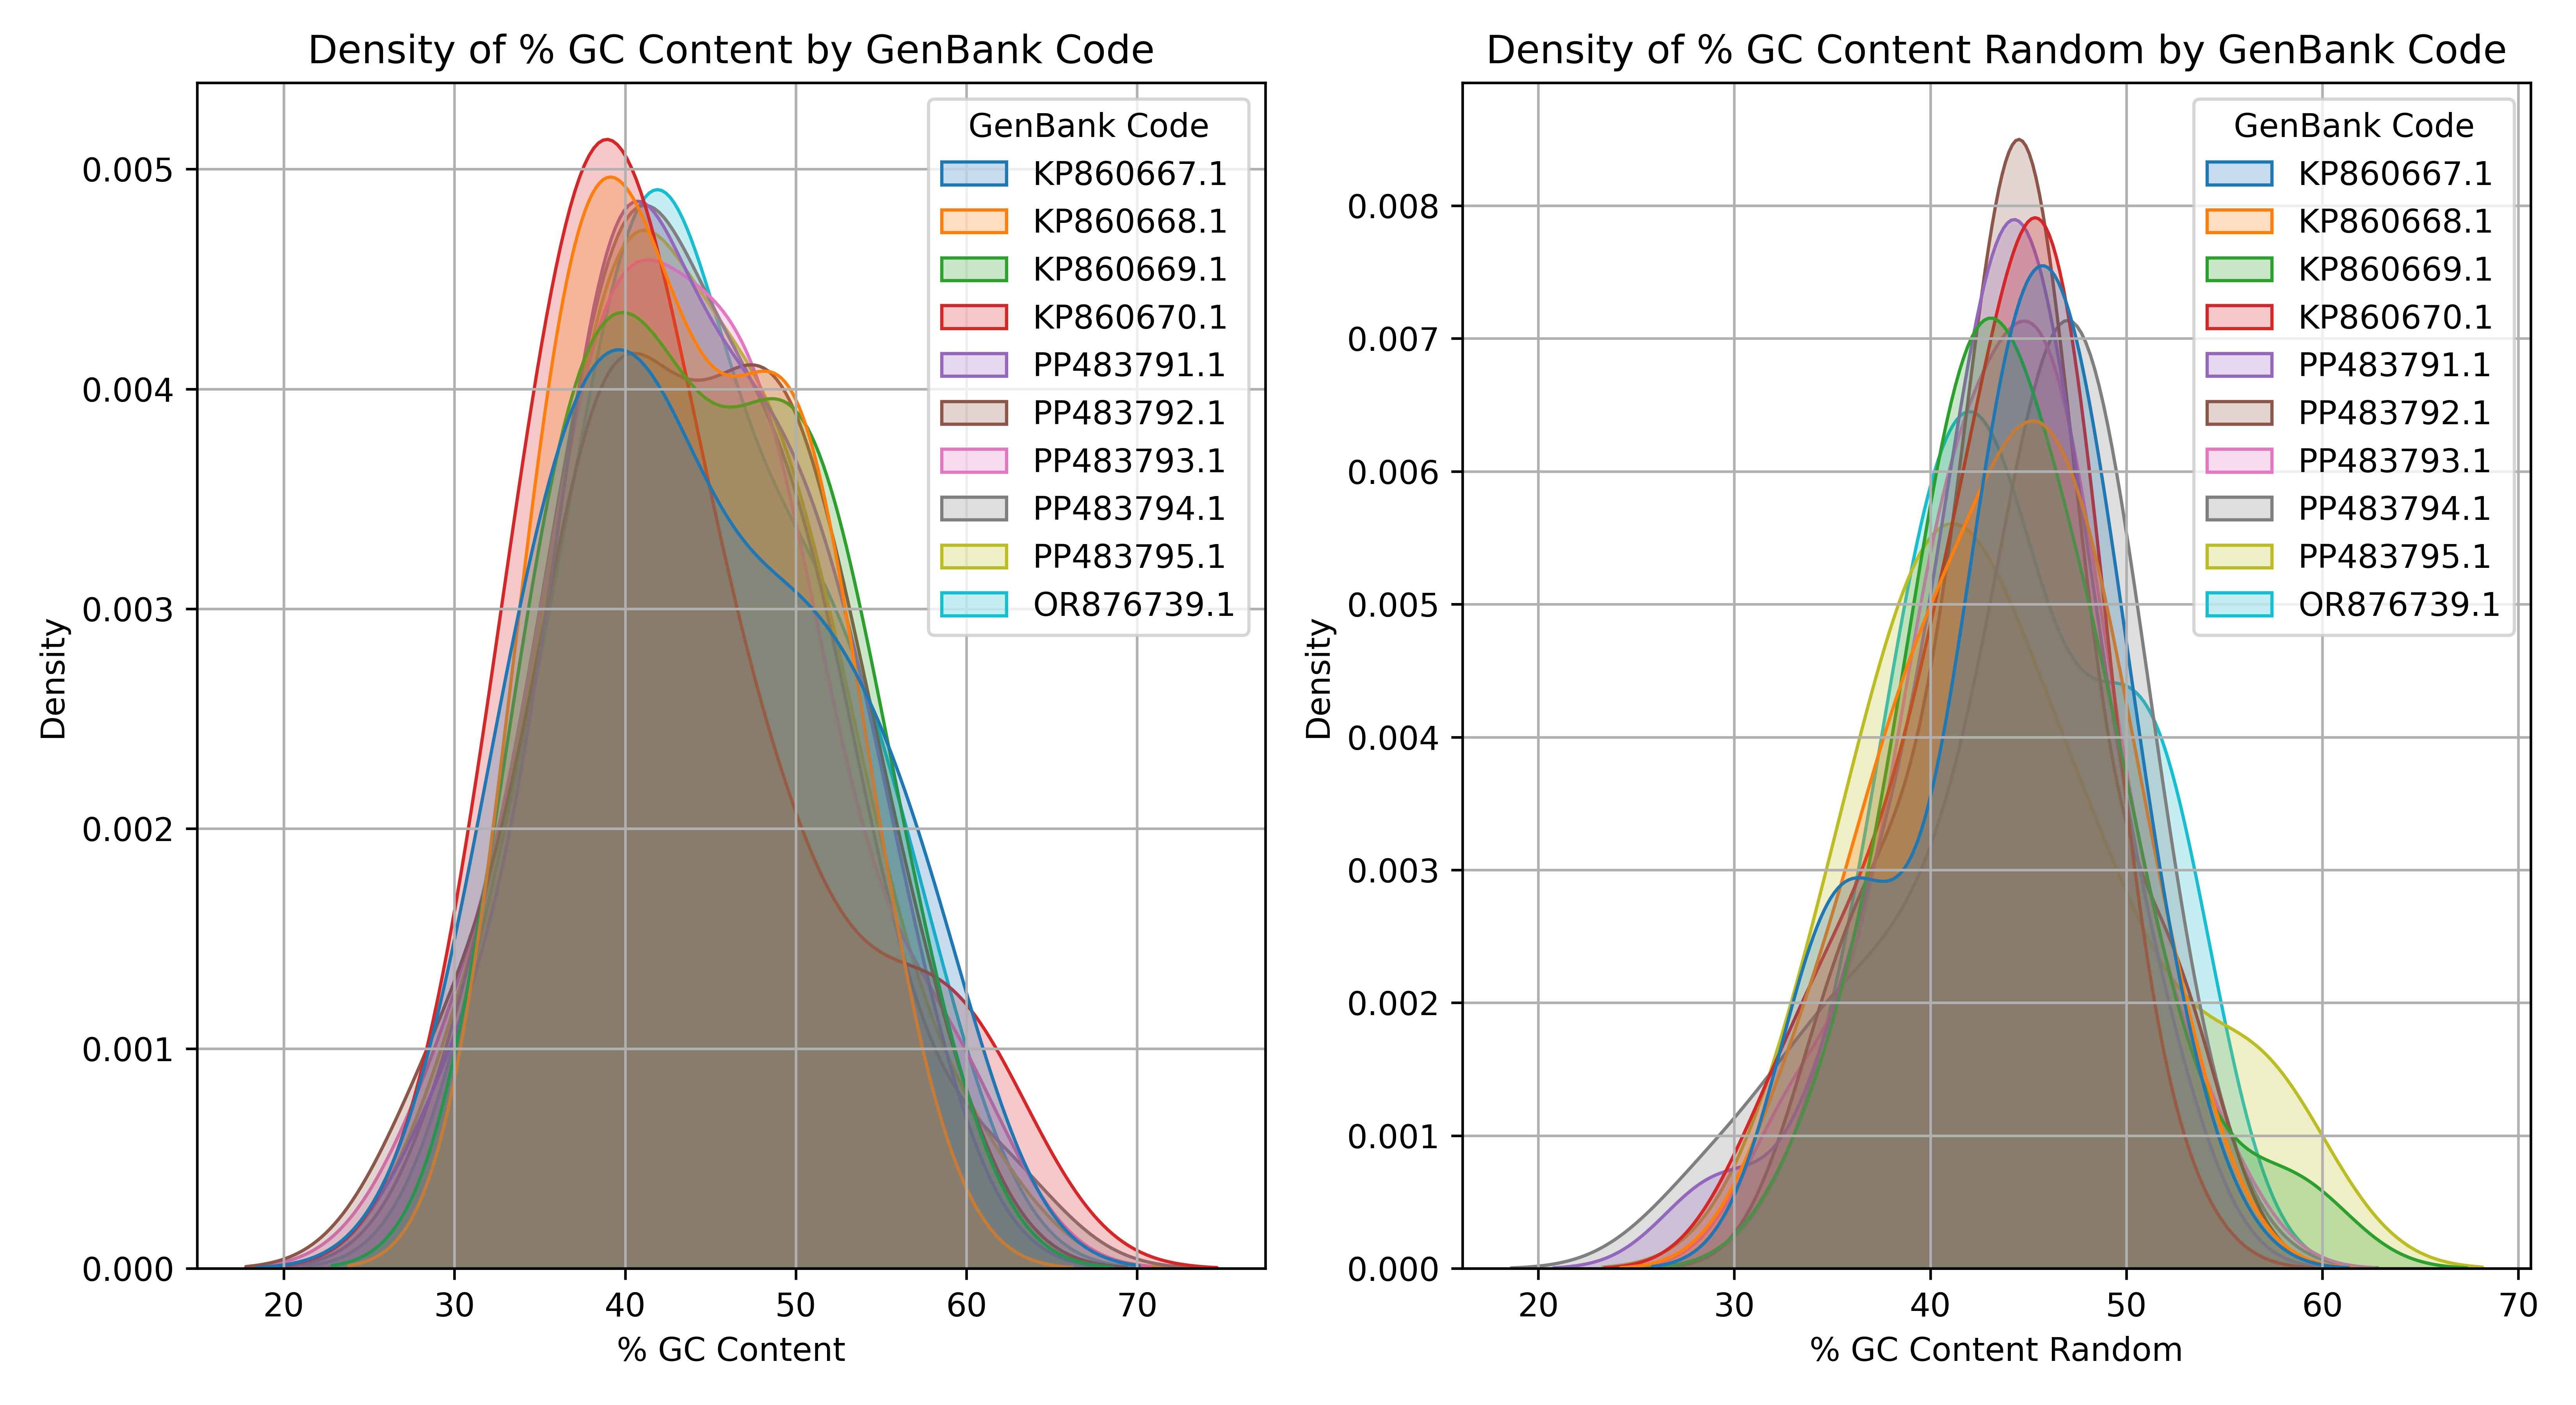
\includegraphics[width=1\textwidth]{density_gc.jpg}%
\caption{Density of \% GC content in the sequences analyzed by fragments at a time.}%
\end{figure}

%
\subsection{Scatterplot of \% GC Content by position and GenBank Code with regression lines}%
\label{subsec:ScatterplotofGCContentbypositionandGenBankCodewithregressionlines}%


\begin{figure}[!htbp]%
\centering%
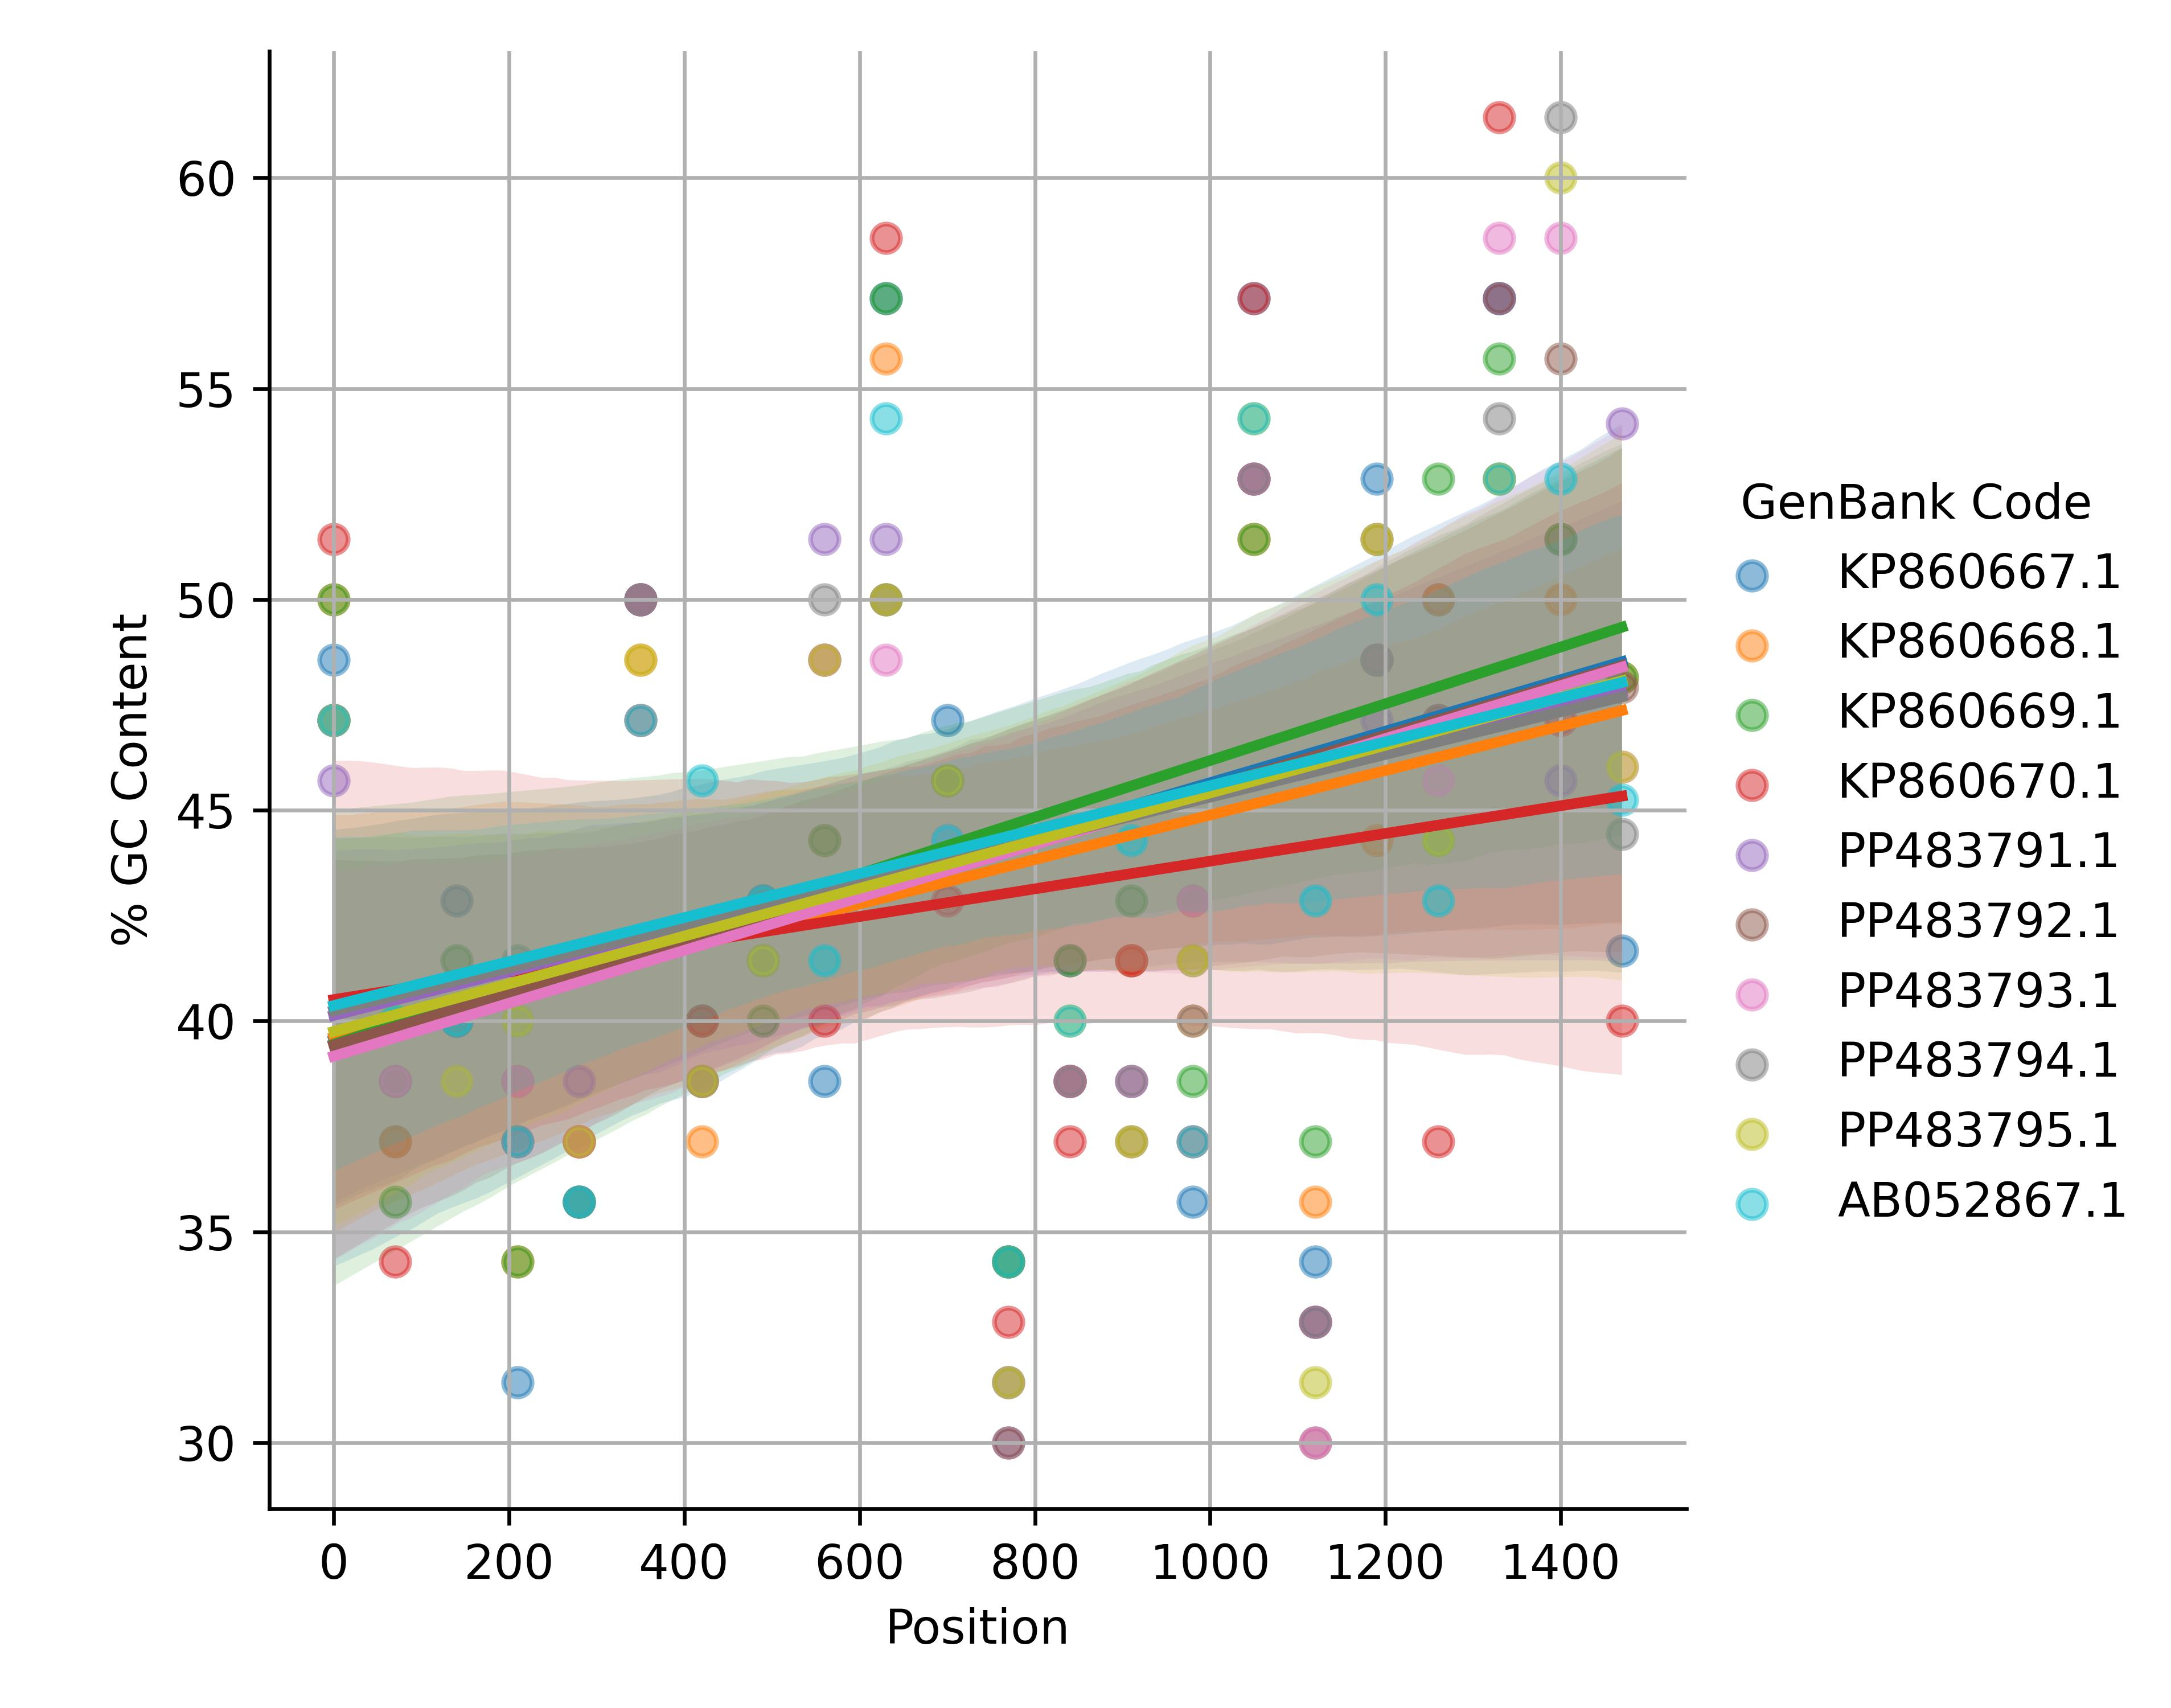
\includegraphics[width=0.8\textwidth]{scatterplot_gc.jpg}%
\caption{Dispersion and regression lines for \% GC Content by position}%
\end{figure}

%
\section{BLASTN Analysis Results}%
\label{sec:BLASTNAnalysisResults}%
The BLASTN analysis was performed to identify homologous sequences to the target sequence within the NCBI nucleotide database. The results were saved in the file blastn\_results.tsv. The columns in the output correspond to: Query sequence ID, Subject sequence ID, Percentage of identical matches, Number of mismatches, Start of alignment in query, End of alignment in query, Alignment length, Start of alignment in subject, End of alignment in subject, Subject sequence length, Subject title, Aligned part of query sequence.\newline%
%
\newline%
The average identity percentage across all alignments is 93.44\%, with a median of 92.67\% and a standard deviation of 2.59\%. The maximum identity percentage found in the BLASTN analysis was 100.00\% and the minimum 91.69\%. %
A statistical test (one{-}sample t{-}test) indicates that the mean identity percentage is higher than 90\% (t = 29.71, p = 0.000000). This supports a strong similarity between the analyzed sequences and the database.%
\subsection{Histogram with density line of BLASTN Identity Percentages}%
\label{subsec:HistogramwithdensitylineofBLASTNIdentityPercentages}%
The following graphic is good for visualizing the frequency at which every percentage of identity is distributed so that the reader can make a more assertive decision based on all previous factors.\newline%
\newline%
 %
The maximum value of identity percentage hits 100\% at least once, hence, a strong conclusion is that the sequence OR876739.1 can be, in fact, a strain of the family of sequences in the database used because it is the same as at least one of them. \newline%
\newline%
In this case, the statistical analysis can be either useless or useful because of this factor, and also as seen in the previous graphics, the similarities are higher than the discrepancies. %


\begin{figure}[!htbp]%
\centering%
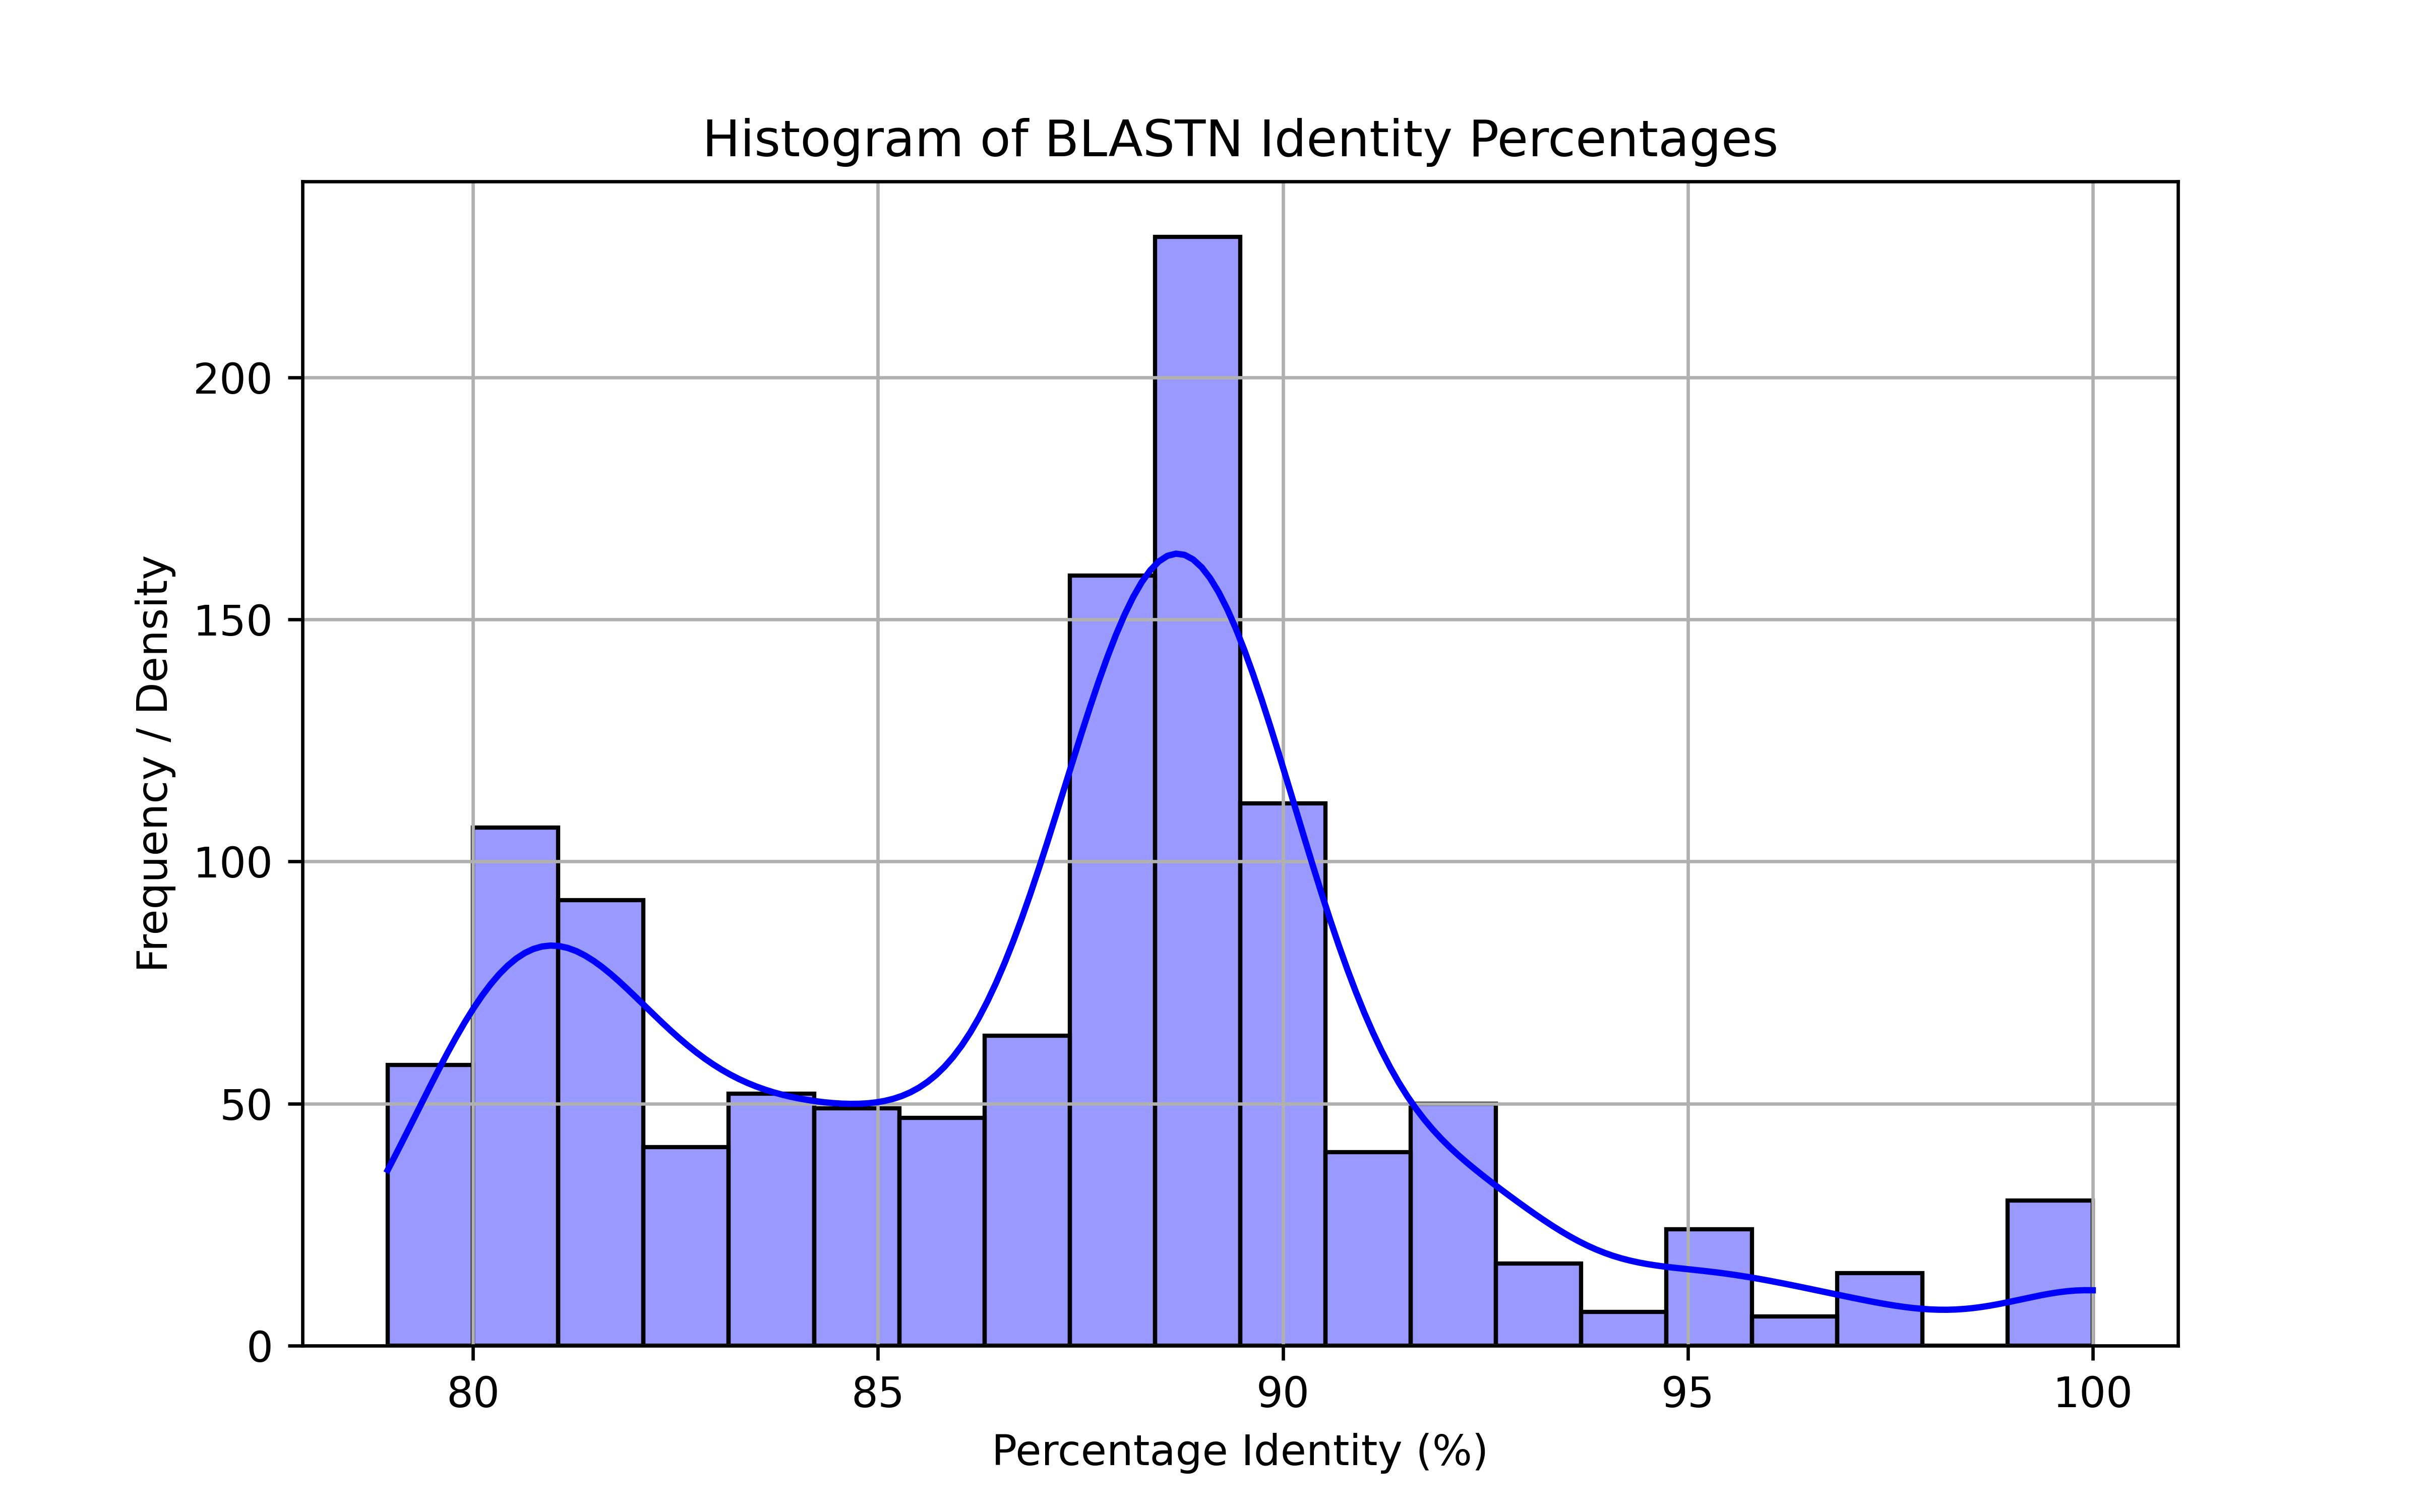
\includegraphics[width=1\textwidth]{hist_kde_pident.jpg}%
\caption{Frequency of identity percentages in BLASTN analysis.}%
\end{figure}

%
PDF generated automatically by: https://github.com/monitoxx/Retrovirus{-}Analyzer{-}V2

%
\end{document}